\task{Мощения}

\begin{itemize}
\itA Из этой фигуры можно собрать горизонтальную полоску ширины 2, которой очевидно можно замостить плоскость (смотреть рисунок).

\begin{center}
	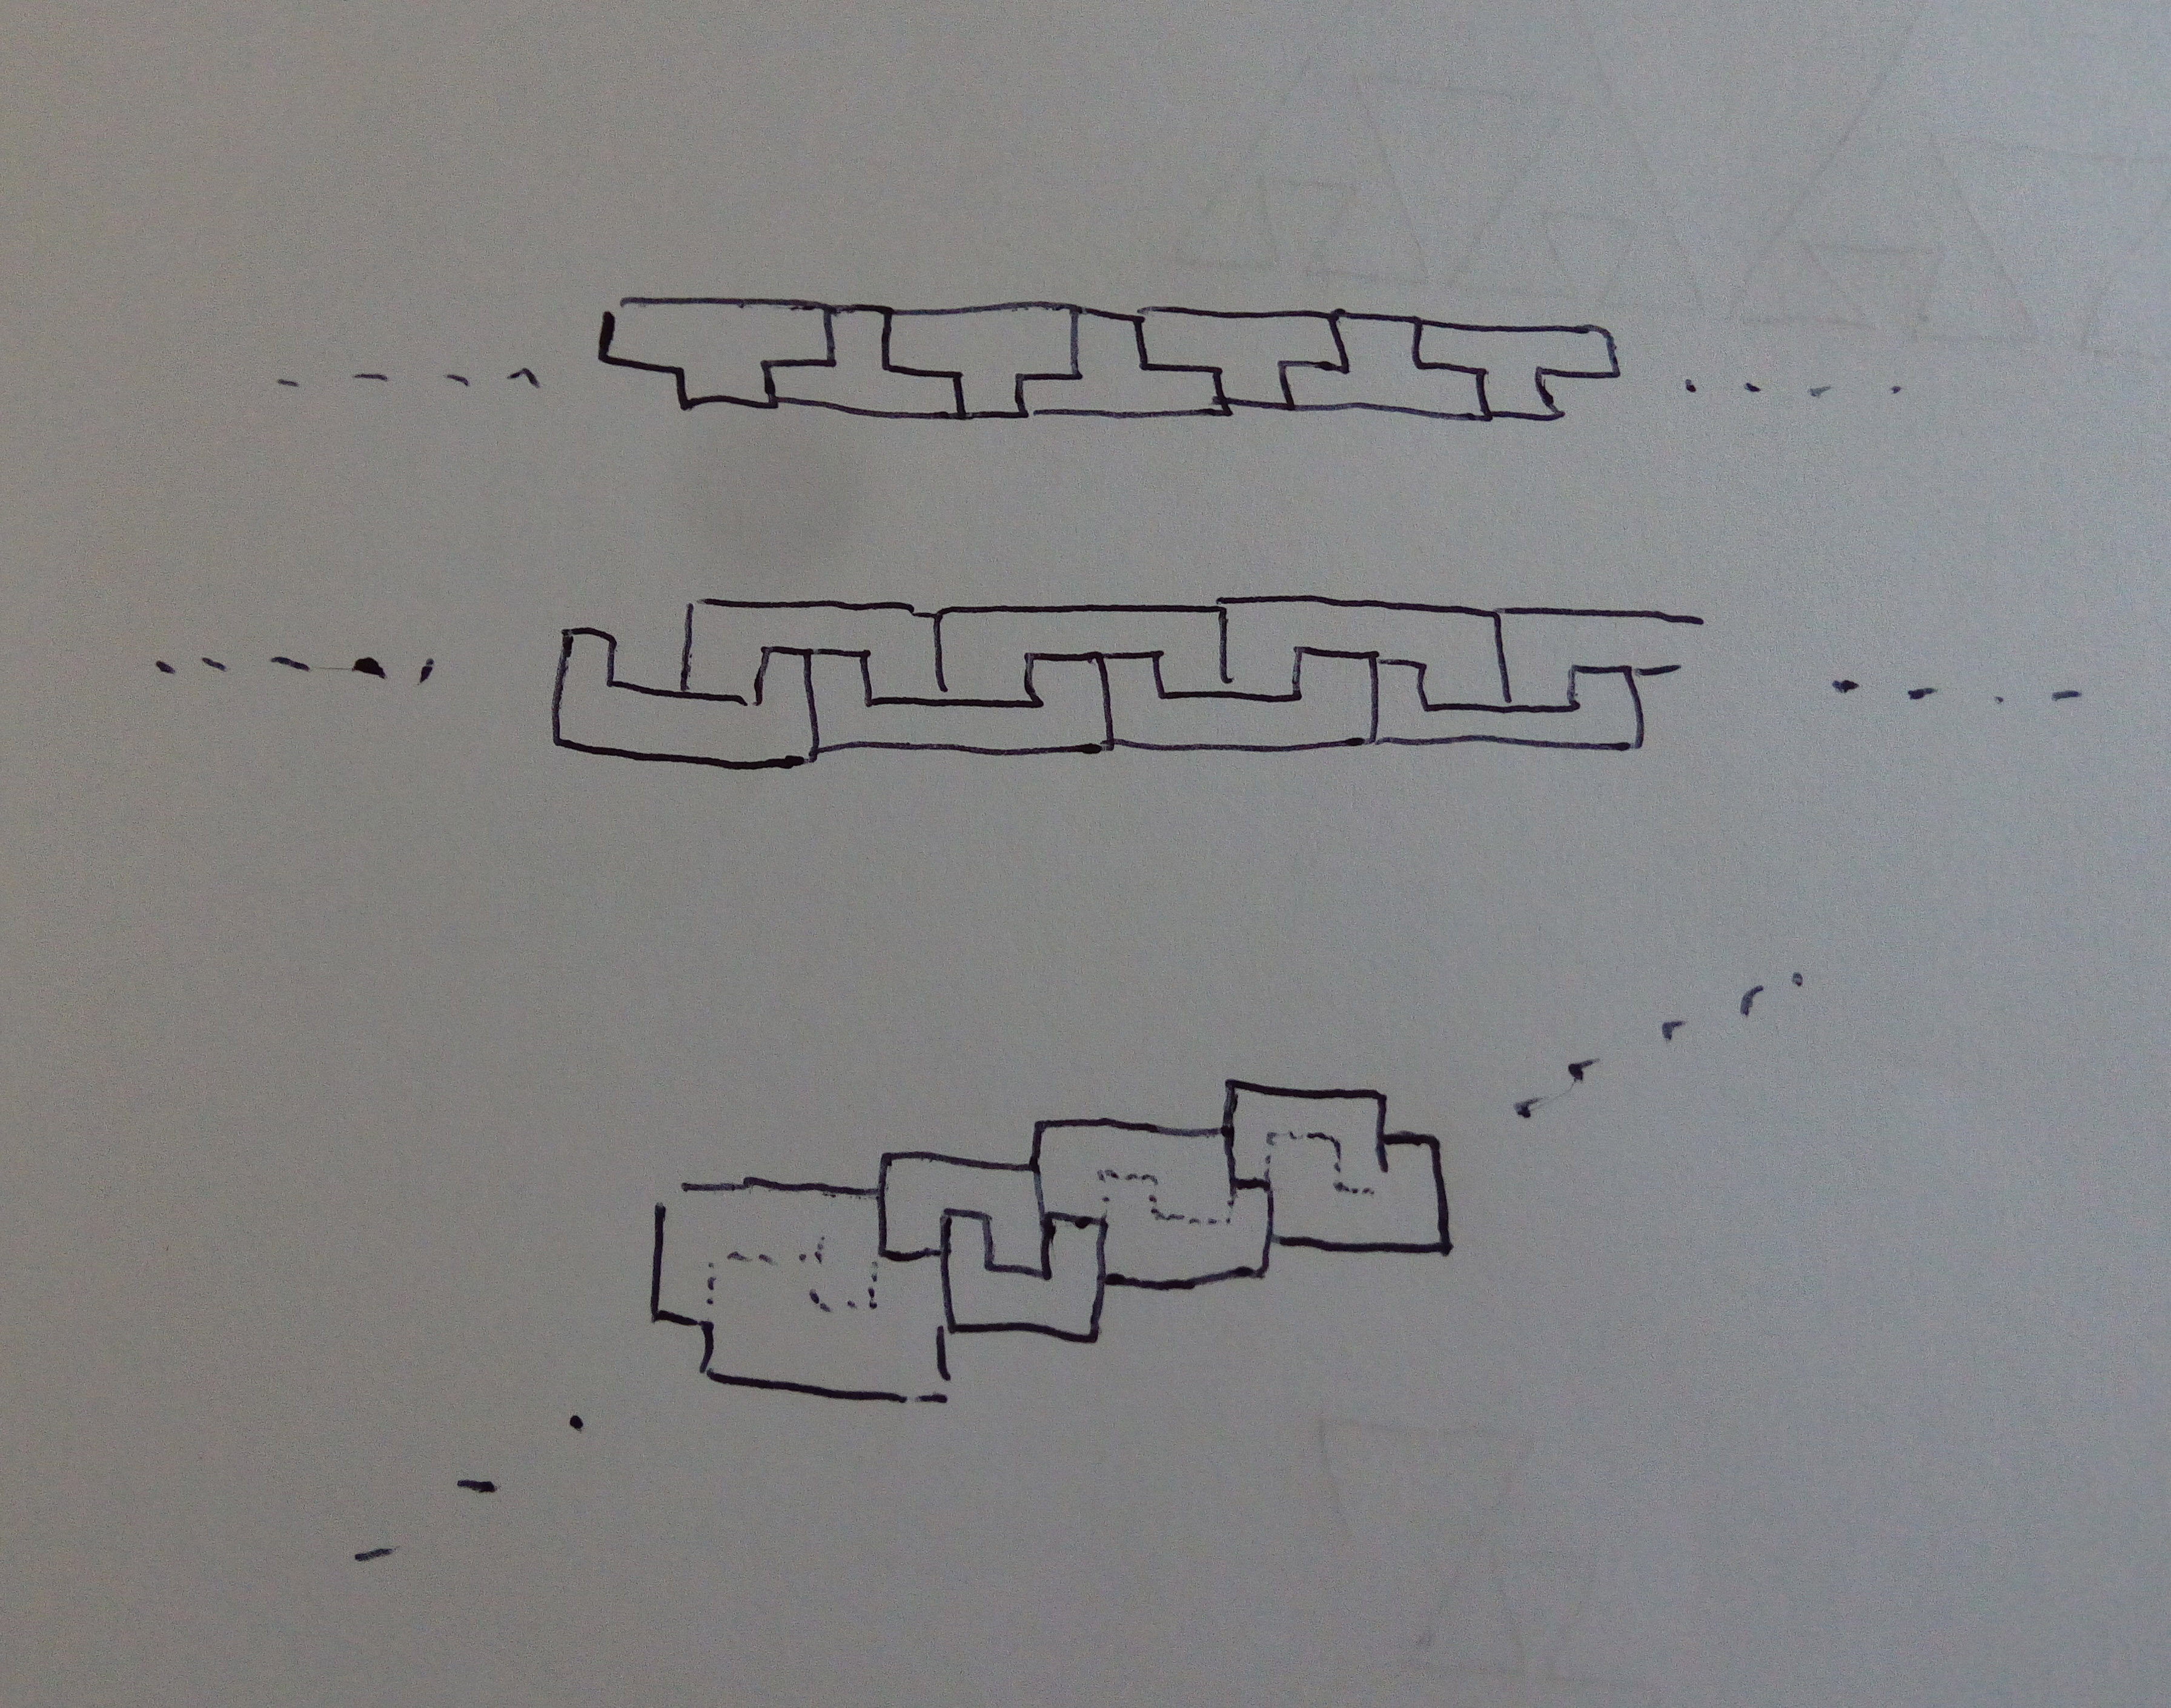
\includegraphics[natwidth=3584,natheight=2820,width=6cm]{figures/2018-plane-park-a}
\end{center}

\itB Из второй фигуры можно собрать горизонтальную полоску ширины 3, которой очевидно можно замостить плоскость. Из первой же фигуры соберём «лесенку» (смотреть рисунок выше): так как и верхний, и нижний её край имеет вид «на три клетки вправо–на клетку вверх», этой лесенкой можно замостить плоскость, прикладывая её к себе.

\itC Смотреть рисунок:
\begin{center}
	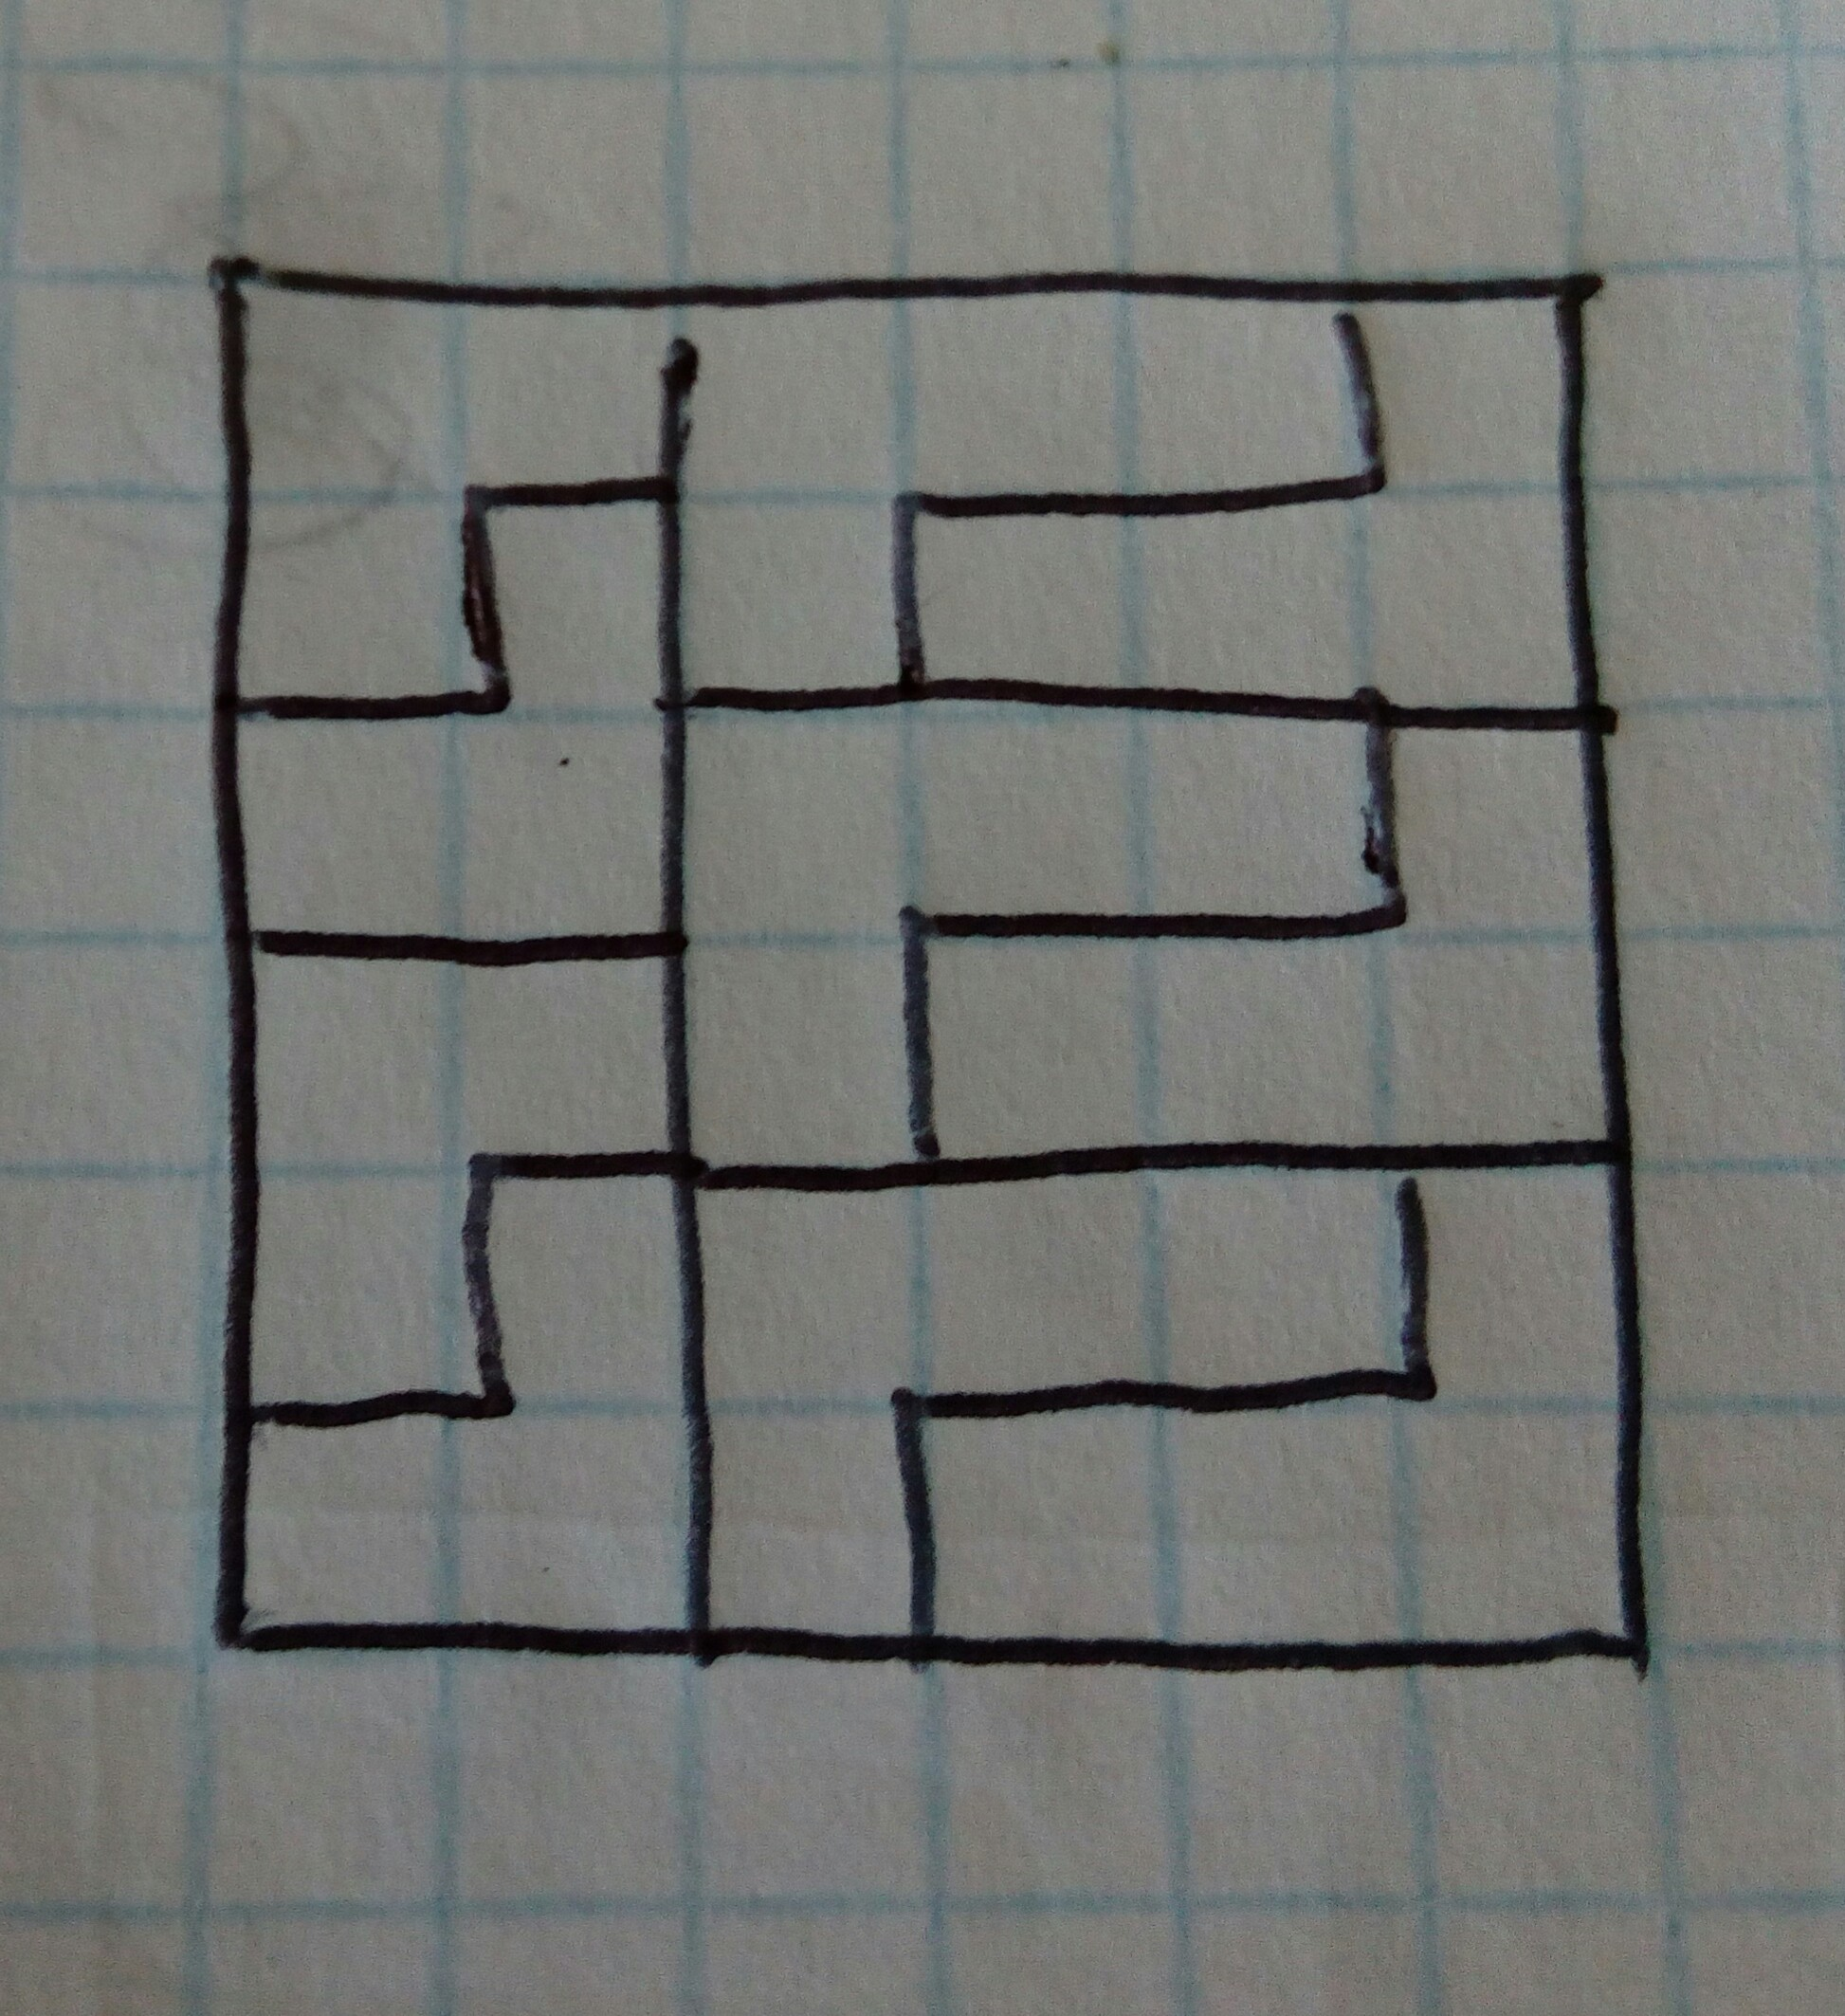
\includegraphics[natwidth=1946,natheight=2126,width=6cm]{figures/2018-plane-park-c}
\end{center}
\end{itemize}